%%%%%%%%%%%%%%%%%%%%
%
% DIRECTIONS
% Students count off 1, 2, 3, ..., 7, do the one question,
% then explain their answer to their neighbor.
% Perhaps volunteers fill out answer key (+doc camera).
%
%%%%%%%%%%%%%%%%%%%%

\RequirePackage{luatex85}
\documentclass[10pt, addpoints]{exam}
\usepackage{tikz, pgfplots, amsmath, mathtools, multicol}
%\pgfplotsset{compat=1.15}
\usepackage[letterpaper, margin=0.5in, column sep=1in]{geometry}
\setlength\parindent{0mm}

% define macro \Repeat{integer}{content}
\usepackage{expl3}
\ExplSyntaxOn
\cs_new_eq:NN \Repeat \prg_replicate:nn
\ExplSyntaxOff

\usepackage{hyperref}

% diagram for questions on pages 1 and 3
\def\yscaleone{3} % = amount to shrink diagram in y direction
\newcommand\diagram{
\fullwidth{
\begin{center}
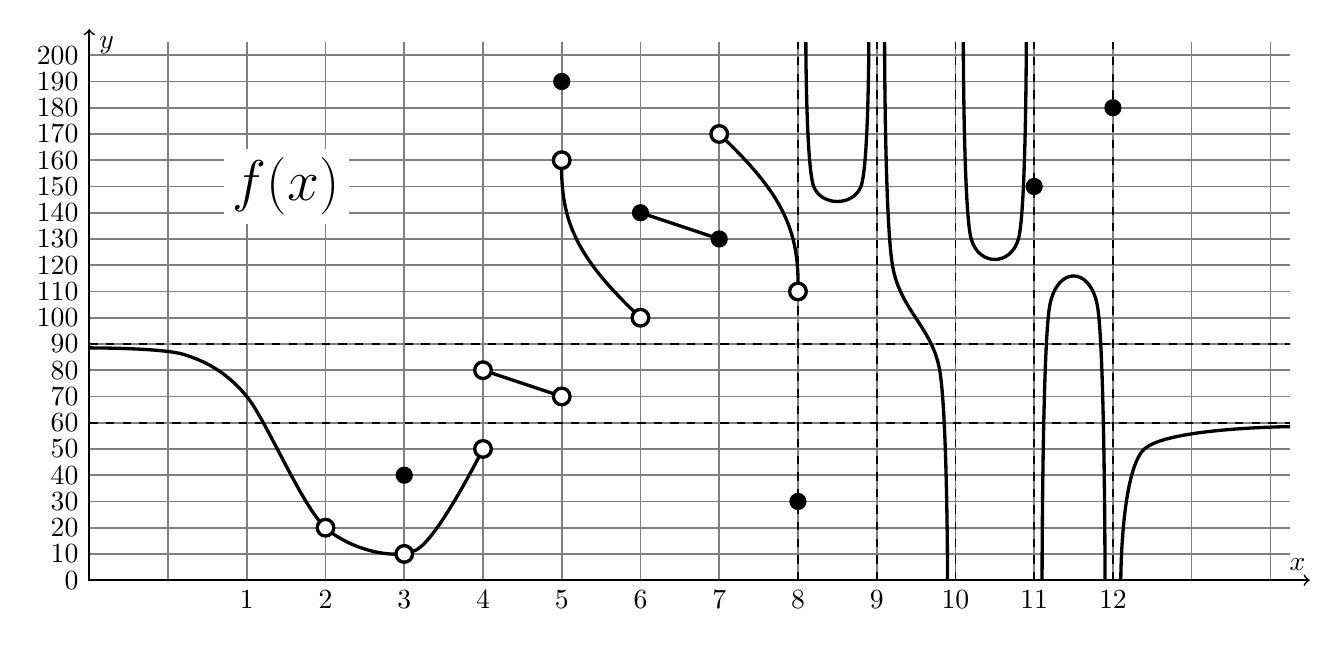
\begin{tikzpicture}
	[very thick, yscale=1/\yscaleone]
	% grid
	\draw[gray, semithick] (-1,0) grid (14.25,20.5);
	% x- and y-axes
	\draw[<->, semithick] (-1,21) -- node[pos=0.03, right] {$y$} (-1,0) -- node[pos=0.99, above] {$x$} (14.5,0);
	% labels on y-axis
	\foreach \y in {0,10,...,200}
	\draw (-1,\y/10) node[left] {\y};
	% labels on x-axis
	\foreach \x in {1,...,12}
	\draw (\x,0) node[below] {\x};
	% vertical asymptotes
	\foreach \x in {8,...,12}
	\draw[dashed, semithick] (\x,0) -- (\x,20.5);
	% horizontal asymptotes
	\foreach \y in {9,6}
	\draw[dashed, semithick] (-1,\y) -- (14.25,\y);
	% plot five curves on left half
	\draw[smooth] plot coordinates{(-1,8.85) (0.2,8.6) (1,7) (2,2) (3.15,1.15) (4,5)};
	\draw (4,8) -- (5,7);
	\draw (5,16) to [bend right=10] (6,10);
	\draw (6,14) -- (7,13);
	\draw (7,17) to [bend left=10]  (8,11);
	% plot five asymptotic curves on right half
	\draw[smooth] plot coordinates {(8.1,20.5) (8.2,15) (8.8,15) (8.9,20.5)};
	\draw[smooth] plot coordinates {(9.1,20.5) (9.2,12) (9.8,8) (9.9,0)};
	\draw[smooth] plot coordinates {(10.1,20.5) (10.2,13) (10.8,13) (10.9,20.5)};
	\draw[smooth] plot coordinates {(11.1,0) (11.2,10.5) (11.8,10.5) (11.9,0)};
	\draw[smooth] plot coordinates {(12.1,0) (12.4,5) (14.25,5.85)};
	% open circles
	\foreach \x/\y in {2/2, 3/1, 4/5, 4/8, 5/7, 5/16, 6/10, 7/17, 8/11}
	\draw[black, fill=white, yscale=\yscaleone] (\x,\y/\yscaleone) circle (3pt);
	% closed circles
	\foreach \x/\y in {3/4, 5/19, 6/14, 7/13, 8/3, 11/15, 12/18}
	\draw[black, fill=black, yscale=\yscaleone] (\x,\y/\yscaleone) circle (2.5pt);
	% f(x) label
	\draw (1.5,15) node[fill,white] {\color{black} \huge$f(x)$};
	\end{tikzpicture}
	\end{center}
	}
	
	\vspace{-1em}
	}

% template for questions 1 through 12 on page 1
\newcommand\threelim{
\question $\left\{\begin{aligned}
	\phantom{\lim_{x\to \mathbf{\arabic{question}}^+}} f(\arabic{question}) &=
	\\[-0.5ex] \lim_{x\to \mathbf{\arabic{question}}^-}f(x) &=
	\\[-0.5ex] \lim_{x\to \mathbf{\arabic{question}}^+}f(x) &=
	\\[-0.5ex] \lim_{x\to \mathbf{\arabic{question}}\phantom{^+}}f(x) &=
	\end{aligned}\right.$}

% template for questions 15 through 26 on page 2
\newcommand\fivelim[4]{
	\question
	\(\begin{matrix}
	\begin{tikzpicture}
	\begin{axis}[
		every axis/.append style={font=\tiny}, 
		xmin=-3.1, xmax=3.1,
		ymin=-2.4, ymax=2.4,
		samples=99, 
		major tick length={0},
		line width=1pt,
		axis lines=center, height=1.6in, width=2in, grid=major,
		restrict y to domain=-2.4:2.4, 
		% title={\normalsize{\unboldmath$\displaystyle f(x) = #1$}},
		extra y tick style={y tick label style={right}},
		#3,
		% samples=59 % speed up compile for testing
		]
		\addplot [black, smooth, thick, domain=-3:3] {#2};
		#4
	\end{axis}
	\end{tikzpicture}
	\end{matrix}\)
	
	\vspace{-3mm}
	\fullwidth{\(\begin{aligned}
		\phantom{\lim_{x\to \mathbf0^+}} f(x) &= \smash{#1}
		\\[-0.9ex] \phantom{\lim_{x\to \mathbf0^+}} f(0) &=
		\\[-0.9ex] \lim_{x\to \mathbf0^-}f(x) &=
		\\[-0.9ex] \lim_{x\to \mathbf0^+}f(x) &=
		\\[-0.9ex] \lim_{x\to \mathbf0\phantom{^+}}f(x) &=
		\\[-0.9ex] \lim_{x\to \mathrlap{-\infty}\phantom{\mathbf0{^+}}}f(x) &=
		\\[-0.9ex] \lim_{x\to \mathrlap{+\infty}\phantom{\mathbf0{^+}}}f(x) &=
		\end{aligned}\)}
	}
\newcommand\fivelima[3]{\fivelim{#1}{#2}{#3}{}}
\newcommand\fivelimb[2]{\fivelima{#1}{#2}{grid=none, ticks=none}}
\newcommand\opencircle[1]{\draw[color=black,fill=white,thick] (axis cs:{#1}) circle [radius=2pt];}

\thispagestyle{empty}
\pagestyle{empty}
\begin{document}
\diagram

\begin{questions}
\section{Finding Limits Graphically}
\begin{multicols}3
\Repeat 7 \threelim
\end{multicols}

\section{Finding Limits Involving Infinity Graphically}
\begin{multicols}3
\Repeat 5 \threelim
\bigskip
\question $\lim\limits_{x\to \mathbf{-\infty}}f(x) =$
\question $\lim\limits_{x\to \mathbf{+\infty}}f(x) =$
\end{multicols}

\clearpage
\section{Famous Functions}
\setlength\columnsep{8mm}
\raggedcolumns
\begin{multicols}4
\fivelimb{1/x}{1/x}
\fivelimb{1/x^2}{1/x/x}
\fivelimb{|x|}{abs(x)}
\fivelim{\sqrt[3]x}{0}{grid=none, ticks=none}{\addplot[black, smooth, thick, domain=-3:3] (x^3,x);}
\end{multicols}

\vfill
\begin{multicols}4
\fivelimb{x^3}{x^3}
\fivelima{e^x}{e^x}{ytick={1}, xtick={0}}
\fivelima{\ln(x)}{ln(x)}{ytick={0}, xtick={1}}
\fivelim{\frac{\left| x \right|}x}{floor(x/10)*2+1}
	{ytick={1},extra y ticks={-1},xtick={0},samples={501}}{\opencircle{0,1} \opencircle{0,-1}}
\end{multicols}

\vfill
\begin{multicols}4
\fivelima{\cos(x)}{cos(deg(x)*2)}{ytick={-1,1},xtick={0}}
%	\fivelim{\frac{\sin(x)}x}{sin(deg(x*3))/(x*3)}{ytick={-1,1},xtick={0}}{\opencircle{0,1}}
\fivelim{\frac{\sin(x)}x}{cos(deg(x*6))*exp(-abs(x/1.25))}{ytick={-1,1},xtick={0}}{\opencircle{0,1}}
\fivelima{\sin(1/x)}{sin(deg(1/x*1.5))}{ytick={-1,1},xtick={0},samples={720}}
\fivelima{x\sin(1/x)}{x/3*sin(deg(1/x*3))}{ytick={-1,1},xtick={0},samples={720}}
\end{multicols}

\newpage
\diagram
\section{Identify Continuity/Discontinuity at a Point} %(removable, jump, infinite)
\question We say $f(x)$ is  \fillin[\textbf{continuous at $x=a$}][2in] 
	if $\lim\limits_{x\to a}f(x)$ exists and equals $f(a)$.
\question We say $f(x)$ has a \fillin[\textbf{removable discontinuity at $x=a$}][2in] at $x=a$ 
	if $\lim\limits_{x\to a}f(x)$ exists and does \emph{not} equal $f(a)$.
\question We say $f(x)$ has a \fillin[\textbf{jump discontinuity at $x=a$}][2in]
	if $\lim\limits_{x\to a^+}f(x)$ and $\lim\limits_{x\to a^-}f(x)$ exist and are \emph{un}equal. 
\question We say $f(x)$ has an \fillin[\textbf{infinite discontinuity at $x=a$}][2in]
	if either $\lim\limits_{x\to a^+}f(x)$ or $\lim\limits_{x\to a^-}f(x)$
	equals either $\infty$ or $-\infty$.

\question The function $f(x)$ is \textbf{continuous at \boldmath $x$ =} \fillin[][3in].
\question The function $f(x)$ is has a \textbf{removable discontinuity at \boldmath $x$ =} \fillin[][3in].
\question The function $f(x)$ is has a \textbf{jump discontinuity at \boldmath $x$ =} \fillin[][3in].
\question The function $f(x)$ is has an \textbf{infinite discontinuity at \boldmath $x$ =} \fillin[][3in].

\section{Identify Left and Right Continuity at a Point}
\question We say $f(x)$ is \fillin[left continuous at $x=a$][3in] if $\lim_{x\to a^-}f(x)$ exists and equals $f(a)$.
\question We say $f(x)$ is \fillin[right continuous at $x=a$][3in] if $\lim_{x\to a^+}f(x)$ exists and equals $f(a)$.

\question The function $f(x)$ is \textbf{left continuous at \boldmath $x$ =} \fillin[][3in].
\question The function $f(x)$ is \textbf{right continuous at \boldmath $x$ =} \fillin[][3in].

\section{Continuity on an Interval}
We say $f(x)$ is \textbf{continuous on \boldmath $(a,b)$}
	if $f(x)$ is continuous at $x=c$ for all $c$ in $(a,b)$.
\question We say $f(x)$ is \textbf{continuous on \boldmath $[a,b]$}
	if $f(x)$ is continuous at $x=c$ for all $c$ in $(a,b)$, \\[3ex]
	and \fillin[right continuous at $x=a$][3in] and \fillin[left continuous at $x=a$][3in].
\question We say $f(x)$ is \textbf{continuous everywhere}
	if $f(x)$ is continuous at $x=c$ for all $c$ in \fillin[][1in].
\question We say $f(x)$ is \textbf{continuous} if it is continuous on every open interval in \fillin[][2.5in].
%\question Identify some intervals on which $f(x)$ is continuous on.
%	Identify some intervals $f(x)$ is \emph{not} continuous on. 
\question Find the union of all open intervals $(a,b)$ such that $f(x)$
	is \textbf{continuous on \boldmath $(a,b)$}. Use interval notation.
%\question Find the domain of $f(x)$. Use interval notation.
\question The function $f(x)$ fails to be \textbf{continuous} (on every open interval in its domain). 
	It fails at $x$ = \fillin[][1.4in].

\end{questions}
\end{document}